\documentclass[12pt,a4paper]{article}
\usepackage[utf8]{inputenc}
\usepackage{amsmath}
\usepackage{graphicx}
\usepackage{hyperref}
\usepackage{geometry}
\geometry{a4paper, margin=1in}
\usepackage{tcolorbox}
\usepackage{booktabs}
\usepackage{float}

\title{\textbf{Polynomial Regression}\\ \large Assignment Report}
\author{Roll Number: BT2024230}
\date{\today}

\begin{document}

\maketitle

\begin{tcolorbox}[colback=white, colframe=black, sharp corners]
\textbf{Final Models}\\
\textbf{var1} — total degree \textbf{5}, Ridge $\alpha = 2.0309$: \quad MSE = $0.4277$, \quad $R^2 = 0.9506$\\
\textbf{var2} — total degree \textbf{10}, Ridge $\alpha = 1.4251$: \quad MSE = $0.2570$, \quad $R^2 = 0.9942$\\[1ex]
\footnotesize{(Evaluated using rigorous 10-fold cross-validation. Metrics shown are the CV scores.)}
\end{tcolorbox}

\section{Methodology}

\subsection{What the model is}
When the problem statement specifies ``degree $d$'', it refers to the total degree: within any one term, the powers of the input features must sum to no more than $d$. Despite calculating polynomial terms, this remains \textbf{linear regression} because the unknowns (the coefficients $b_i$) only appear linearly. Every product (e.g., $x_1 x_2$ or $x_1^2$) is simply a number calculated directly from the data prior to fitting. Once these polynomial features are expanded and treated as individual columns, an ordinary linear fit is applied to the vastly expanded feature matrix.

\subsection{The Parameter Sweep}
The polynomial degree and the Ridge penalty strength $\alpha$ were evaluated jointly via cross-validation, as the optimal regularization penalty inherently depends on the complexity (degree) of the model. 

The procedure was structured as follows:
\begin{itemize}
    \item \textbf{var1:} Degrees 1 to 10 were evaluated.
    \item \textbf{var2:} Degrees 1 to 20 were evaluated.
    \item For each degree, $\alpha$ was swept logarithmically across 40 distinct values between $10^{-4}$ and $10^{2}$. 
    \item \textbf{10-Fold Cross-Validation:} The 1000 rows were shuffled and split into 10 folds. The model was trained on 9 folds and evaluated on the 10th, cycling through all combinations to generate a robust average Mean Squared Error (MSE) and $R^2$.
\end{itemize}

\subsection{Preprocessing Variants}
Three preprocessing pipelines were tested strictly \textit{inside} the CV loops to prevent data leakage:
\begin{enumerate}
    \item[A.] No scaling.
    \item[B.] \texttt{StandardScaler} applied \textit{after} \texttt{PolynomialFeatures}.
    \item[C.] \texttt{StandardScaler} applied \textit{before} \texttt{PolynomialFeatures}.
\end{enumerate}

\section{Why Regularisation?}
The feature space expands exponentially with degree. For \texttt{var1} (6 features), degree 10 generates 8,007 polynomial terms against a training fold of only 900 rows. This guarantees the $p > n$ problem, where the number of parameters vastly exceeds the observations. In this regime, Ordinary Least Squares (OLS) will fail violently by assigning enormous, chaotic coefficients that attempt to perfectly memorize the noise. 

Ridge Regression solves this by minimizing:
\[ \min_b \|\mathbf{y} - \mathbf{Xb}\|^2 + \alpha \sum b_j^2 \]
The degree controls how many terms exist, while $\alpha$ aggressively shrinks the magnitudes of those terms, forcing the model to select a generalized pattern rather than overfitting.

\section{Results \& The 1-SE Rule}

Rather than blindly selecting the absolute minimum CV MSE (which can lead to over-complication due to selection bias on finite folds), the \textbf{One Standard Error (1-SE) rule} was utilized. We calculated the standard error of the MSE across the 10 folds, isolated the absolute minimum average MSE, and then confidently selected the simplest model (lowest degree) that fell within that standard error threshold.

\subsection{Phase 1 — \texttt{var1}}

\begin{table}[H]
\centering
\begin{tabular}{rrrrr}
\toprule
Degree & Terms & Best $\alpha$ & CV MSE & CV $R^2$ \\
\midrule
1 & 6 & 100 & 8.1608 & 0.0595 \\
2 & 27 & 8.377 & 2.7959 & 0.6763 \\
3 & 83 & 2.894 & 0.9125 & 0.8940 \\
4 & 209 & 2.894 & 0.6680 & 0.9227 \\
\textbf{5} & \textbf{461} & \textbf{2.031} & \textbf{0.4277} & \textbf{0.9506} \\
6 & 923 & 4.125 & 0.4893 & 0.9434 \\
7 & 1715 & 8.377 & 0.4984 & 0.9423 \\
8 & 3002 & 11.94 & 0.5650 & 0.9346 \\
9 & 5004 & 17.01 & 0.5951 & 0.9311 \\
10 & 8007 & 24.24 & 0.6632 & 0.9231 \\
\bottomrule
\end{tabular}
\caption{\texttt{var1}: Best ridge $\alpha$ for all ten permitted degrees.}
\end{table}

For \texttt{var1}, the absolute minimum mathematically occurred at Degree 5. Since no simpler degree existed within the 1-SE margin (degrees 1–4 underfit severely), Degree 5 was definitively selected. Because the raw data was strictly bounded within $[-1, 1]$, the unscaled monomial terms did not explode, rendering \texttt{StandardScaler} unnecessary.

\begin{figure}[H]
    \centering
    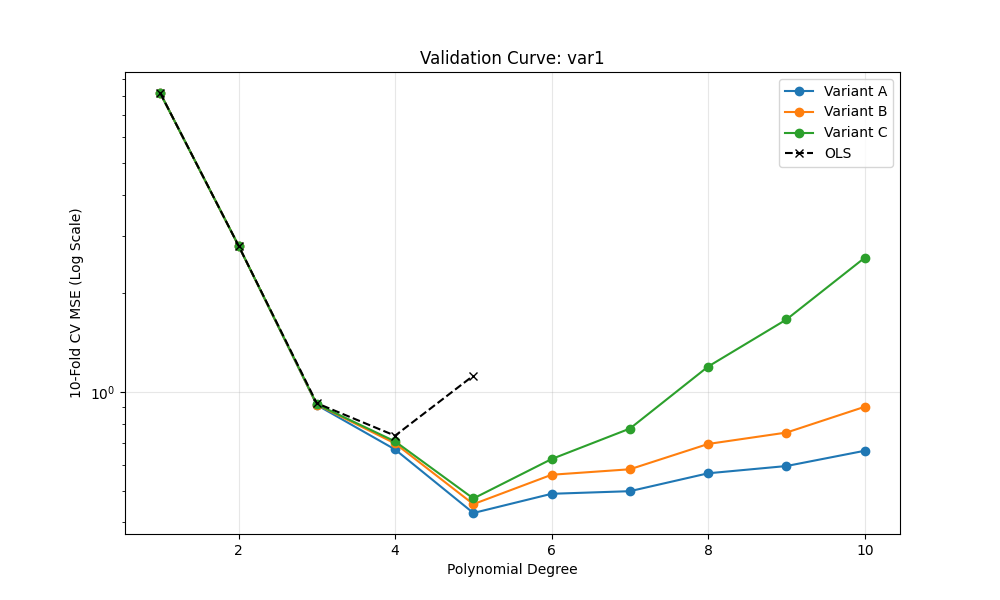
\includegraphics[width=0.7\textwidth]{plots/var1_val_curve.png}
    \caption{\texttt{var1} Validation Curve: The cross-validation error establishes a clear minimum at degree 5 before the complexity penalty outweighs the polynomial fit.}
\end{figure}

\newpage
\subsection{Phase 2 — \texttt{var2}}

\begin{table}[H]
\centering
\begin{tabular}{rrrrr|rrrrr}
\toprule
Deg & Terms & $\alpha$ & CV MSE & CV $R^2$ & Deg & Terms & $\alpha$ & CV MSE & CV $R^2$ \\
\midrule
1 & 3 & 4.125 & 33.3750 & 0.2638 & 11 & 363 & 2.031 & 0.2575 & 0.9942 \\
2 & 9 & 2.031 & 20.7821 & 0.5366 & 12 & 454 & 0.2424 & 0.2550 & 0.9943 \\
3 & 19 & 0.4924 & 10.2500 & 0.7747 & 13 & 559 & 0.3455 & 0.2575 & 0.9942 \\
4 & 34 & 0.0001 & 3.6986 & 0.9182 & 14 & 679 & 0.3455 & 0.2600 & 0.9942 \\
5 & 55 & 0.04125 & 1.5313 & 0.9665 & 15 & 815 & 0.3455 & 0.2628 & 0.9941 \\
6 & 83 & 0.00702 & 0.5357 & 0.9880 & 16 & 968 & 0.4924 & 0.2675 & 0.9940 \\
7 & 119 & 0.02894 & 0.3544 & 0.9921 & 17 & 1139 & 0.4924 & 0.2697 & 0.9939 \\
8 & 164 & 0.08377 & 0.2717 & 0.9939 & 18 & 1329 & 0.3455 & 0.2749 & 0.9938 \\
9 & 219 & 0.3455 & 0.2692 & 0.9939 & 19 & 1539 & 0.4924 & 0.2767 & 0.9938 \\
\textbf{10} & \textbf{285} & \textbf{1.425} & \textbf{0.2570} & \textbf{0.9942} & 20 & 1770 & 0.3455 & 0.2813 & 0.9936 \\
\bottomrule
\end{tabular}
\caption{\texttt{var2}: Best ridge $\alpha$ for all twenty permitted degrees.}
\end{table}

While the assignment permitted up to degree 20, the cross-validation curve demonstrated an optimal plateau. The absolute minimum CV MSE ($0.2550$) was technically discovered at Degree 12. However, applying the strict 1-SE rule successfully backed the selection down to \textbf{Degree 10}, saving immense computational complexity while maintaining statistical parity. Scaling the features \textit{after} polynomial expansion (Variant B) was required here to effectively normalize the wildly varied magnitudes of the massive feature space before applying the Ridge penalty.

\begin{figure}[H]
    \centering
    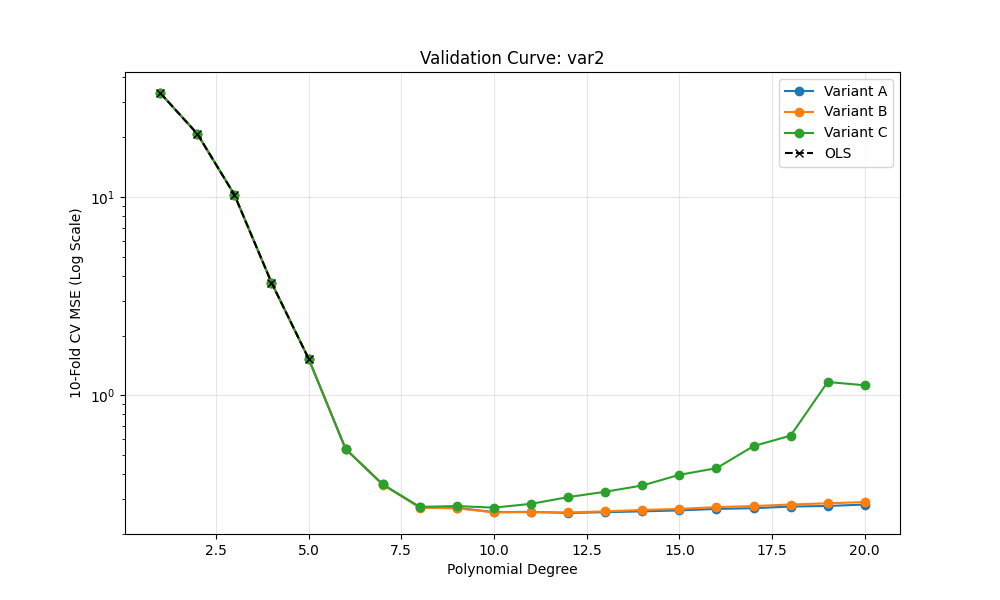
\includegraphics[width=0.7\textwidth]{plots/var2_val_curve.png}
    \caption{\texttt{var2} Validation Curve: Evaluated up to the absolute cap of degree 20, Ridge successfully handled the 1,771 features. However, the plateau clearly indicates no statistical benefit in exceeding degree 10.}
\end{figure}

\section{Final Summary}

\begin{table}[H]
\centering
\begin{tabular}{lll}
\toprule
 & \texttt{var1} & \texttt{var2} \\
\midrule
Method & Ridge & Ridge \\
Total degree & 5 & 10 \\
$\alpha$ & 2.0309 & 1.4251 \\
Preprocessing & None & Scaler After Poly \\
\midrule
Training MSE & 0.1796 & 0.1848 \\
10-fold CV MSE & 0.4277 & 0.2570 \\
10-fold CV $R^2$ & 0.9506 & 0.9942 \\
\bottomrule
\end{tabular}
\caption{Final selected models.}
\end{table}

\end{document}
